\documentclass[9pt]{beamer}
\usepackage{silence}
\WarningFilter{beamerthememetropolis}{You need to compile with XeLaTeX or LuaLaTeX to use the Fira fonts}
\usetheme[titleformat = smallcaps, block = fill, progressbar = frametitle]{metropolis}
\title{\Huge Mathematics - Introduction}
%---------------------------------%
% PACKAGES
%---------------------------------%
% Input encoding.
\usepackage[utf8]{inputenc} % For accents in spanish: transforms "á" into "\'a"
\usepackage[T1]{fontenc} % Output encoding. Use to avoid silly problems on the output.
                         % See: http://tex.stackexchange.com/questions/664/why-should-i-use-usepackaget1fontenc
\usepackage[sfdefault]{FiraSans}
\usepackage{FiraMono}
% AMS packages
\usepackage{amsmath}
\usepackage{amsfonts}
\usepackage{amssymb}
\usepackage{amsthm}
% Matrices
\usepackage{mathtools}
\newcommand{\verteq}{\rotatebox{90}{$\,=$}}
\usepackage{gauss}
% Customization for augmented matrices; 
% see https://tex.stackexchange.com/questions/146723/how-to-typeset-row-operations-on-augmented-matrix
% Patch gauss macros for doing their work in `align'
% and other amsmath environments; see http://tex.stackexchange.com/questions/146532/
\usepackage{etoolbox}
\makeatletter
\patchcmd\g@matrix
    {\vbox\bgroup}
    {\vbox\bgroup\normalbaselines} % restore the standard baselineskip
    {}{}
\makeatother
\newcommand{\BAR}{%
    \hspace{-\arraycolsep}%
    \strut\vrule % the `\vrule` is as high and deep as a strut
    \hspace{-\arraycolsep}%
}
% Math blackboard font
\usepackage{bbm}
% Fonts
\usepackage{lmodern} 
% \usepackage[sfdefault]{FiraSans}
\usepackage[normalem]{ulem}
\usepackage{eulervm}
% Graphics
\usepackage{graphicx} 
\usepackage{float}
\usepackage{subcaption}
\usepackage{wrapfig}
\usepackage{animate}
\usepackage{caption}
% Algorithms
\usepackage[ruled]{algorithm2e}
\newcommand{\lIfElse}[3]{\lIf{#1}{#2 \textbf{else}~#3}}
% Boxes
\usepackage[most]{tcolorbox}
% For reference enumerations lists
\usepackage{enumitem}
% \setlist{labelwidth = \widthof{0.}, leftmargin = {\labelwidth+\labelsep}, 
%         rightmargin = \leftmargin} % Setting left marging = right marging in itemize envirnment
% Import icons
\usepackage{fontawesome}
% Hyperlink
\usepackage{hyperref}
\hypersetup{
	final,
    bookmarksnumbered=true,
    bookmarksopen=true,
    bookmarksopenlevel=0,
    unicode=false,          % non-Latin characters in Acrobat?s bookmarks
    pdftoolbar=true,        % show Acrobat?s toolbar?
    pdfmenubar=true,        % show Acrobat?s menu?
    pdffitwindow=false,     % window fit to page when opened
    pdftitle={Introduction to Mathematics},    % title
    pdfdisplaydoctitle=true, %display document title instead of file name in title bar
    pdftoolbar=true,
    pdfmenubar=true,
    pdflang={English},
    pdfauthor={Abel Guada Azze},     % author
    pdfsubject={Introduction to Mathematics},   % subject of the document
    pdfcreator={Abel Guada Azze},   % creator of the document
    pdfproducer={Abel Guada Azze}, % producer of the document
    pdfkeywords={Mathematics} {introduction}, % list of keywords
    pdfnewwindow=true,      % links in new window
    breaklinks=true,
    hidelinks,
    colorlinks,
    linkcolor=black,          % color of internal links (change box color with linkbordercolor)
    citecolor=black,        % color of links to bibliography
    filecolor=cyan,      % color of file links
    urlcolor=magenta           % color of external links
}
%----------------------------------- Tikz
\usepackage{tikz}
\usepackage{pgfplots}
% \pgfplotsset{compat=1.18}
% \usepackage{tkz-euclide}
\usetikzlibrary{shapes,arrows.meta,matrix,positioning,calc}
\newcommand{\tikzmark}[1]{\tikz[baseline,remember picture] \coordinate (#1) {};}
% ---------- Helpers: 2-set and 3-set Venns ----------
% \VennTwoCounts{LabelA}{LabelB}{onlyA}{both}{onlyB}{Neither}{Universe}
\newcommand{\VennTwoCounts}[7]{%
  \begin{tikzpicture}[scale=1.0,baseline=(current bounding box.center)]
    \def\r{1.8}   % circle radius (cm)
    \def\dx{2.35} % distance between centres (cm)
    \def\pad{0.60} % padding between circles and rectangle (cm)

    \coordinate (A) at (0,0);
    \coordinate (B) at (\dx,0);

    % Universe rectangle (outline only)
    \draw[line width=.8pt, rounded corners=2pt]
      ($(A)+(-\r-\pad,-\r-\pad)$) rectangle ($(B)+(\r+\pad,\r+\pad)$);

    % Set fills + outlines
    \fill[black!8] (A) circle (\r);
    \fill[black!8] (B) circle (\r);
    \draw[line width=.8pt] (A) circle (\r);
    \draw[line width=.8pt] (B) circle (\r);

    % Universe label (top-left inside the box)
    \node[font=\scriptsize,anchor=north west]
      at ($(A)+(-\r-\pad+0.12,\r+\pad-0.12)$) {#7};

    % Set labels
    \node[font=\small\bfseries] at ($(A)+(0,0.68*\r)$) {#1};
    \node[font=\small\bfseries] at ($(B)+(0,0.68*\r)$) {#2};

    % Counts
    \node[font=\small] at ($ (A)+(-0.60*\r,-0.05*\r) $) {#3}; % only A
    \node[font=\small] at ($ .5*(A)+.5*(B) $) {#4};           % both
    \node[font=\small] at ($ (B)+(0.60*\r,-0.05*\r) $) {#5};  % only B
    \node[font=\small]
      at ($ (B)+(\r+0.3*\pad,0.78*\r) $) {#6};                % outside
  \end{tikzpicture}%
}


%---------------------------------%
% Biblio
%---------------------------------%

%---------------------------------%
% SETTINGS
%---------------------------------%
% displays sections and subsections numbered in the TOC
\setbeamertemplate{section in toc}[sections numbered]
% \setbeamertemplate{subsection in toc}[subsections numbered]
% gets rid of bottom navigation bars
\setbeamertemplate{footline}{}
% gets rid of bottom navigation symbols
\setbeamertemplate{navigation symbols}{}
% sets images' path
\graphicspath{{img/}}
% resets footnote counter at the beginning of each section
\AtBeginEnvironment{frame}{\setcounter{footnote}{0}}
% beamer margins
\setbeamersize
{
    text margin left=3mm,
    text margin right=3mm,
    % sidebar width left=.0cm,
    % sidebar width right=.0cm,
    % description width,
    % description width of=,
    % mini frame size=,
    % mini frame offset
}
% redefines block environment to add small space between title and content
\let\oldblock\block
\let\endoldblock\endblock
\renewenvironment{block}[1]
    {\begin{oldblock}{#1}
        \vspace{0.1cm}
    }
    { 
    \end{oldblock}
    }

%---------------------------------%
% SETTINGS
%---------------------------------%
%---------------------------------%
% TITLE PAGE
%---------------------------------%
\setbeamertemplate{title page}{
    \vspace{-0.4cm}
    
    \textcolor{CUNEForange}{\rule{\textwidth}{0.05cm}}
    \vspace{-0.65cm}
    
    \begin{minipage}{0.2\textwidth}
        \includegraphics[width = 2.0cm]{Logo-CUNEF.png}
    \end{minipage}
    \begin{minipage}{0.7\textwidth}
        
        \quad \Huge \usebeamertemplate*{title}
        
    \end{minipage}    
    \vspace{-0.25cm}
    
    \textcolor{CUNEForange}{\rule{\textwidth}{0.05cm}}
    \vspace{1.5cm}

    \begin{minipage}{0.075\textwidth}
        
    \end{minipage}\hfill\textcolor{CUNEForange}{\vrule\vrule\vrule}
    \begin{minipage}{0.825\textwidth}
        \begin{itemize}[leftmargin = *, label= $ $]
            \item {\hspace{1.05pt} \faUser\quad Abel Guada Azze}
            \item {\hspace{0pt} \faEnvelope\quad \href{mailto:abel.guada@cunef.edu}{abel.guada@cunef.edu}}
            \item {\hspace{0pt} \faSuitcase\quad F4.5 - C. de Leonardo Prieto Castro, 2}
            \item {\hspace{0pt} \faUniversity\ \ \ Department of Quantitative Methods - CUNEF Universidad}
            \item {\hspace{0pt} \faGraduationCap\ \ \ Bachelor in Philosophy, Politics and Economics}
        \end{itemize}
    \end{minipage}
}
\setbeamertemplate{title}{
  \linespread{1.0}%
  \inserttitle%
  \par%
  \vspace*{0.5em}
}
\setbeamertemplate{subtitle}{
  \insertsubtitle%
  \par%
  \vspace*{0.5em}
}
\titlegraphic{
\includegraphics[height = 2.0cm]{logo-CUNEF.png}}	
\author[]{Abel G. Azze}
\institute[]{Department of Quantitative Methods \\ CUNEF Universidad}
\date{}
%---------------------------------%
% TITLE PAGE
%---------------------------------%
%---------------------------------%
% CUSTOM COMMANDS AND DEFINITIONS
%---------------------------------%
% define new colors
\definecolor{amber}{rgb}{1.0, 0.49, 0.0}
\definecolor{firebrick3}{RGB}{207, 33, 32}
\definecolor{deepskyblue3}{RGB}{0, 155, 206}
\definecolor{darkorange3}{RGB}{206, 102, 0}
\definecolor{darkolivegreen3}{RGB}{163, 207, 91}
\definecolor{CUNEForange}{RGB}{237, 114, 1}
\definecolor{CUNEFblue}{RGB}{36, 51, 71}
\definecolor{background-gray}{RGB}{251, 251, 250}
\definecolor{block-background-gray}{RGB}{229, 230, 230}
% coloring commands
\newcommand{\red}[1]{\textcolor{firebrick3}{#1}}
\newcommand{\black}[1]{\textcolor{black}{#1}}
\newcommand{\blue}[1]{\textcolor{deepskyblue3}{#1}}
\newcommand{\green}[1]{\textcolor{darkolivegreen3}{#1}}
\newcommand{\orange}[1]{\textcolor{darkorange3}{#1}}
\newcommand{\purple}[1]{\textcolor{purple}{#1}}
\newcommand{\Corange}[1]{\textcolor{CUNEForange}{#1}}
\newcommand{\Cblue}[1]{\textcolor{CUNEFblue}{#1}}
% footnote without number
\newcommand\footnotenonum[1]{%
  \begingroup
  \renewcommand\thefootnote{}\footnote{#1}%
  \addtocounter{footnote}{-1}%
  \endgroup
}
% hyperbolic secant
\DeclareMathOperator{\sech}{sech}
\DeclareMathOperator{\csch}{csch}
% Plain macros
\newcommand{\N}{\mathbb{N}} % natural number set
\newcommand{\Z}{\mathbb{Z}} % entire number set
\newcommand{\Q}{\mathbb{Q}} % rational number set
\newcommand{\R}{\mathbb{R}} % real number set
\newcommand{\I}{\mathbb{I}} % imaginary number set
\newcommand{\cF}{\mathcal{F}} % sigma-algebra
\newcommand{\cD}{\mathcal{D}} % stopping set
\newcommand{\cX}{\mathcal{X}} % bridge sets
\newcommand{\cC}{\mathcal{C}} % continuation set
\newcommand{\cB}{\mathcal{B}} % ball around a point
\newcommand{\cA}{\mathcal{A}} % subset of R+xR
\newcommand{\cR}{\mathcal{R}} % compact set
\newcommand{\cN}{\mathcal{N}} % normal distribution
\newcommand{\rmd}{\mathrm{d}} % differential operator
\newcommand{\rmb}{\mathsf{b}} % OSB of the original OSP
\newcommand{\rK}{\mathsf{K}} % Kernel of the original OSP
\newcommand{\rPhi}{\mathsf{\Phi}} % Phi of the original OSP
\newcommand{\rphi}{\mathsf{\boldsymbol{\phi}}} % Phi of the original OSP
\newcommand{\InfGen}{\mathbb{L}} % infinitesimal generator
\newcommand{\InfGenOr}{\mathsf{L}} % infinitesimal generator. Original version
\newcommand{\Ind}{\mathbbm{1}} % indicator function
\newcommand{\lp}{\left(} % left parenthesis
\newcommand{\rp}{\right)} % right parenthesis
\newcommand{\lb}{\left[} % left brackets
\newcommand{\rb}{\right]} % right brackets
\newcommand{\lc}{\left\{} % left curly brackets
\newcommand{\rc}{\right\}} % right curly brackets
\newcommand{\blp}{\big(}
\newcommand{\brp}{\big)}
\newcommand{\blb}{\big[}
\newcommand{\brb}{\big]}
\newcommand{\blc}{\big\{}
\newcommand{\brc}{\big\}}
% Macros with arguments
\newcommand\redsout{\bgroup\markoverwith{\textcolor{red}{\rule[0.5ex]{2pt}{0.4pt}}}\ULon}
\newcommand\bluesout{\bgroup\markoverwith{\textcolor{blue}{\rule[0.5ex]{2pt}{0.4pt}}}\ULon}
\newcommand{\lrav}[1]{\left|#1\right|} % absolute value
\newcommand{\wt}[1]{\widetilde{#1}}
\newcommand{\wh}[1]{\widehat{#1}}
\newcommand{\ol}[1]{\overline{#1}}
\newcommand{\ul}[1]{\underline{#1}}
\newcommand{\lrp}[1]{\lp#1\rp} % left-right parenthesis
\newcommand{\lrb}[1]{\lb#1\rb} % left-right brackets
\newcommand{\lrc}[1]{\lc#1\rc} % left-right curly brackets
\newcommand{\blrp}[1]{\blp#1\brp} % big left-right parenthesis
\newcommand{\blrb}[1]{\blb#1\brb} % big left-right brackets
\newcommand{\blrc}[1]{\blc#1\brc} % big left-right curly brackets
\newcommand{\Prob}[1]{\mathbb{P}\lp #1\rp} % probability 1
\newcommand{\Pro}[2]{\mathbb{P}_{#2}\lp #1\rp} % probability 2
\renewcommand{\Pr}{\mathbb{P}} % probability 3
\newcommand{\PProb}[1]{\mathsf{P}\lp #1\rp} % probability 1.2
\newcommand{\PPro}[2]{\mathsf{P}_{#2}\lp #1\rp} % probability 2.2
\newcommand{\PPr}{\mathsf{P}} % probability 3.2
\newcommand{\Esp}[1]{\mathbb{E}\lb #1\rb} % mean 1
\newcommand{\Espbigg}[1]{\mathbb{E}\bigg[\!#1\bigg]} % mean 1 bigg
\newcommand{\Es}[2]{\mathbb{E}_{#2}\lb #1\rb} % mean 2
\newcommand{\Esbigg}[2]{\mathbb{E}_{#2}\bigg[\!#1\bigg]} % mean 2 bigg
\newcommand{\E}{\mathbb{E}} % mean 3
\newcommand{\EEsp}[1]{\mathsf{E}\lb #1\rb} % mean 1.2
\newcommand{\EEs}[2]{\mathsf{E}_{#2}\lb #1\rb} % mean 2.2
\newcommand{\EE}{\mathsf{E}} % mean 3.2
\newcommand{\V}[1]{\mathbb{V}\mathrm{ar}\lb #1\rb} % variance 1
\newcommand{\Vs}[2]{\mathbb{V}\mathrm{ar}_{#2}\lb #1\rb} % variance 2
\newcommand{\VV}[1]{\mathrm{V}\mathrm{ar}\lb #1\rb} % variance 1 original OSP
\newcommand{\VVs}[2]{\mathrm{V}\mathrm{ar}_{#2}\lb #1\rb} % variance 2 original OSP
\newcommand{\Cov}[2]{\mathbb{C}\mathrm{ov}\lb #1,#2\rb} % covariance
\newcommand{\CCov}[2]{\mathsf{C}\mathrm{ov}\lb #1,#2\rb} % covariance original OSP
%---------------------------------%
% CUSTOM COMMANDS AND DEFINITIONS
%---------------------------------%



%----------------------------- -------------- -----------------------------%
%----------------------------- BEGIN DOCUMENT -----------------------------%
%----------------------------- -------------- -----------------------------%
\begin{document}
%----------------------- TITLE -----------------------%
\maketitle
%----------------------- TITLE -----------------------%
% \begin{frame}{Course overview}

%     \textbf{This course is designed to help you understand the foundations of Mathematics} and build a strong basis for further subjects in the bachelor in Philosophy, Politics and Economics (PPE)
%     \vspace{0.2cm}
    
%     The course will cover a range of basic topics, including \textbf{algebra, calculus, geometry, and differential equations}, but more than anything it aims to \textbf{teach you problem-solving and reasoning skills}
%     \vspace{0.2cm}
    
%     Through numerous examples and problems, the course emphasizes \textbf{the application of mathematics to economy}
    
% \end{frame}

\begin{frame}{Some organizational issues}

    \textbf{E-mail:} \Corange{abel.guada@cunef.edu}
    \vspace{0.2cm}
    
    \textbf{Office hours:} either in person or via Google Meet (send an email beforehand!)
    
    \vspace{0.2cm}
    \textbf{Evaluation:} 
    \begin{itemize}
        \item[$\bullet$] Continuous evaluation ($40\%$)
        \begin{itemize}
            \item[-] Quizzes at the end of each topic ($10\%$)
            \item[-] 1st midterm ($15\%$)
            \item[-] 2nd midterm ($15\%$)
        \end{itemize}
        \item[$\bullet$] Final exam ($60\%$)
        \begin{itemize}
            \item[-] Covers all topics 
            \item[-] Minimum grade is $5$!
        \end{itemize}
    \end{itemize}
    
\end{frame}

% \begin{frame}{Understanding the grading system}

%     \begin{block}{Grades}
%     The following marks will be important throughout the course:    
%     \begin{minipage}{0.4\textwidth}
%         \vspace{-0.3cm}
%         \begin{itemize}[leftmargin=1cm,label=$\bullet$]
%             \item $AR$: attendance rate
%             \item $Q$: quizzes
%             \item $M1$: 1st midterm
%             \item $M2$: 2nd midterm
%         \end{itemize}
%     \end{minipage}
%     \begin{minipage}{0.55\textwidth}
%         \vspace{0.27cm}
%         \begin{itemize}[leftmargin=*,label=$\bullet$]
%             \item $CE_O$: continuous evaluation in ordinary call
%             \item $CE_R$: continuous evaluation in retake call
%             \item $FE$: final exam grade
%             \item $RE$: retake exam grade
%             \item $FG$: final grade
%         \end{itemize}
%     \end{minipage}
%     \end{block}

    % \textbf{Evaluation:} 
    % \vspace{-0.3cm}
    
    % \begin{itemize}
    %     \item[$\bullet$] Continuous evaluation ($40\%$)
    %     \begin{itemize}
    %         \item[-] Quizzes at the end of each topic ($10\%$)
    %         \item[-] 1st midterm ($15\%$)
    %         \item[-] 2nd midterm ($15\%$)
    %     \end{itemize}
    %     \item[$\bullet$] Final exam ($60\%$)
    %     \begin{itemize}
    %         \item[-] Covers all topics 
    %         \item[-] Minimum grade is $5$!
    %     \end{itemize}
    % \end{itemize}    
    
    % \begin{algorithm}[H]
    %     $CE_O = 0.1Q + 0.15M1 + 0.15M2$ \\
    %     \uIf{$AR < 0.8$}{$FE = 0$}
    %     \lIfElse{$FE \geq 5$}{$FG = 0.4CE_O + 0.6FE$}{$FG = FE$}
    %     \uIf{$RE \geq 5$}{
    %         $CE_R = \max(0.4CE_O + 0.6FE, FE)$ \\
    %         $FG = 0.4CE_R + 0.6RE$            
    %     }\uElse{
    %         $FG = RE$
    %     }
    %     \caption{Final grade calculator}
    % \end{algorithm}

% \begin{center}
% \vspace{-0.15cm}
  
% \sffamily
% \begin{tikzpicture}[auto, 
%     block_custom/.style = {rectangle, draw = black, rounded corners = 0.1cm, thick},
%     block_D/.style ={rectangle, draw = deepskyblue3, rounded corners = 0.1cm, thick},
%     block_V/.style ={rectangle, draw = darkolivegreen3, rounded corners = 0.1cm, thick},
%     block_noborder/.style ={rectangle, draw = none, thick, fill = none,
%                             text width = 1mm, text centered, minimum height = 1mm},
%     block_title/.style ={rectangle, draw = none, thick, fill = none,
%                          text centered},        
%     line/.style ={draw, thick, shorten >=0pt},
%     arrow/.style ={draw, thick, -latex', shorten >=0pt}
%     ]
    
%     \matrix [column sep = 2.4cm, row sep = 0.7cm, ampersand replacement = \&, yshift = 2cm] {
      
%         \node [block_custom] (AR) {
%         AR: attendance rate
%         }; \\
%     };
    
%     \matrix [column sep = 1cm, row sep = 0.7cm, ampersand replacement = \&, yshift = 0cm] {
        
%         \node [block_custom] (CE1) {
%         $
%         \begin{aligned}
%             \text{Q:} &\text{ Quizzes} \\
%             \text{M1:}  &\text{ 1st midterm} \\
%             \text{M2:} &\text{ 2nd midterm}
%         \end{aligned}
%         $
%         }; \&
        
%         \node [block_custom] (FE) {
%         FE: final exam
%         }; \\
%     };
    
%     \matrix [column sep = 1.5cm, row sep = 0.7cm, ampersand replacement = \&, yshift = -2cm] {

%         \node [block_custom] (CE2) {
%         $\text{CE } = 0.1\text{Q } + 0.15\text{M1 } + 0.15\text{M2 }$
%         }; \&

%         \node [block_custom] (RE) {
%         RE: resit exam
%         }; \\
%     };
    
%     \matrix [column sep = 1cm, row sep = 0.7cm, ampersand replacement = \&, yshift = -3.5cm] {
        
%         \node [block_custom] (FG1) {
%         $\text{FG } = \max(0.4\text{CE } + 0.6\text{FE}, FE)$
%         }; \&
        
%         \node [block_custom] (FG2) {
%         $\text{FG } = \text{ RE}$
%         }; \\
%     };
    
%     \matrix [column sep = 3cm, row sep = 0.7cm, ampersand replacement = \&, yshift = -4.5cm,  xshift = 1cm] {
%         \node [block_custom] (pass) {
%         Passed :)
%         }; \&
%         \node [block_custom] (not-pass) {
%         Didn't pass :(
%         }; \\
%     };    
    
%     \begin{scope}[every path/.style=arrow]
%         \path (AR) -- ++ (1.8, 0) -| coordinate[pos = 0.75] (AR_l1) (FE);
%         \path (AR) -- ++ (3, 0) -| coordinate[pos = 0.75] (AR_l2) (RE);
%         \path (FE) -- coordinate[pos = 0.45, xshift = -0.1cm] (FE_l1) ++ (0, -2.7) -| (FG1);
%         \path (FE) -- ++ (0, -0.7) -| coordinate[pos = 0.25] (FE_l2) (RE);
%         \path (CE2) -- ++ (0, -0.7) -| coordinate[midway] (CE_l2) (FG1);
%         \path (CE1) --  ([xshift = 0.27cm]CE2.north);
%         \path[-] (FG2) -- coordinate[midway] (FG) (FG1);
%         \path (FG) |- coordinate[pos = 0.7] (pass_l) (pass);
%         \path (FG) |- coordinate[pos = 0.72] (not-pass_l) (not-pass);
%         \path (RE) -- coordinate[midway] (resit1) (FG2);
%     \end{scope}

%     \node [right] at (AR_l1) {$\text{AR} \geq 0.8$};
%     \node [left] at (FE_l1) {$\text{FE} \geq 5$};
%     \node [below] at (FE_l2) {$\text{FE} < 5$};
%     \node [right] at (AR_l2) {$\text{AR} < 0.8$};    
%     \node [below] at (pass_l) {$\text{FG} \geq 5$};
%     \node [above] at (not-pass_l) {$\text{FG} < 5$};
    
% \end{tikzpicture}
% \end{center}
% \end{frame}

\begin{frame}
\frametitle{More organizational issues}
\centering
{\huge\alert{\textbf{EVERYTHING}} is in \alert{\textbf{CANVAS}}}
\vspace{1.5cm}

\hspace{0.3cm}
\begin{minipage}{0.3\textwidth}
\begin{itemize}
    \item[$\bullet$] Midterm exams dates
    \item[$\bullet$] Grades
\end{itemize}
\end{minipage}
\begin{minipage}{0.3\textwidth}
\begin{itemize}
    \item[$\bullet$] Quizzes
    \item[$\bullet$] Teaching material
\end{itemize}
\end{minipage}
\begin{minipage}{0.3\textwidth}
\begin{itemize}
    \item[$\bullet$] Syllabus
    \item[$\bullet$] Announcements
\end{itemize}
\end{minipage}
% \begin{minipage}{0.45\textwidth}
%     \centering
%     \includegraphics[width=0.5\textwidth]{img/canvas_logo.png}
% \end{minipage}
\end{frame}

\begin{frame}{Even more organizational issues}

    \begin{itemize}[leftmargin = 0.5cm, label = $\bullet$]

    \item \textbf{Speaking in class}: You can only speak to contribute something to the class or to ask a question. People who disrupt the class will be expelled from the classroom. \medskip

    \item \textbf{Mobile phones}: must remain in the backpack/bag during the class. \medskip

    \item \textbf{Laptops}: can be used for taking notes, performing specific computations, or taking the course quizzes. \medskip

    \item \textbf{Punctuality}: You cannot enter the classrooms once the class has started.

    \end{itemize}
    
\end{frame}

\begin{frame}{Quizzes}

    \begin{itemize}[leftmargin = 0.5cm, label = $\bullet$]

    \item There will be \textbf{four quizzes} that make \textbf{$10\%$ of your final grade} \medskip

    \item The quizzes will be taken \textbf{at the end of each module}\medskip

    \item You cannot take the quiz at home\medskip

    \item You will need your \textbf{laptop} with the \textbf{chrome browser} and \textbf{Proctorio} installed, and a reliable \textbf{internet connection} \medskip

    \item Check this video on \href{https://www.youtube.com/watch?v=GpYY2GSPfp8}{how to install Proctorio} on Canvas\medskip

    \item There is a \textbf{``Dummy Quiz'' in Canvas} that you can take to check if Proctorio is running OK \medskip

    \item \textbf{It is you responsibility} to be on time and ready to take the quiz, otherwise you will be graded as zero.

    \end{itemize}
    
\end{frame}

% \begin{frame}{What is Mathematics?}

%     \begin{block}{What Mathematics is not about}
%         Mathematics is \Corange{NOT} about \Corange{numbers, formulas, shapes, equations, algorithms}... \\
%         just as Literature is not about words, sentences, metaphors, grammar...
%     \end{block}
    
%     \begin{block}{What Mathematics is about (Máthēma: that which is learned)}
%         Mathematics is about \Corange{understanding}. It is a universal \Corange{language} for expressing \Corange{ideas} and \Corange{solving problems} across various disciplines, including science, engineering, economics, and others. 
%     \end{block}

%     \begin{minipage}{0.53\textwidth}
%         \begin{block}{Skills of Mathematics}
%             \vspace{0.1cm}
            
%             \begin{itemize}[leftmargin = 0.5cm, label = $\bullet$]
%                 \item Decision making 
%                 \item Optimization
%                 \item Analysis
%                 \item The recognition and study of patterns
%                 \item Problem solving
%                 \item Connecting ideas using logic and reason
%             \end{itemize}
%         \end{block}
%     \end{minipage}
%     \begin{minipage}{0.05\textwidth}
%         {\hspace{0cm} }
%     \end{minipage}
%     \begin{minipage}{0.37\textwidth}
%         \vspace{0.1cm}
        
%         \begin{tcolorbox}[enhanced,sharp corners,
%             width = {4.5cm},
%             colback = white,
%             overlay = {\node[circle, fill, background-gray] at (frame.south east) {\faQuoteRight};
%             \node at (frame.south east) {\faQuoteRight};
%             \node[circle, fill, background-gray] at (frame.north west) {\faQuoteLeft};
%             \node at (frame.north west) {\faQuoteLeft};} ]
%             Mathematics is not so much a subject as a way of studying any subject \\
%             \vspace{0cm}
            
%             {\small - George FJ. Temple}
%         \end{tcolorbox}
%         % {\centering
%         % {\large
        
%         %     $^{\text{\faQuoteLeft}}$ Mathematics is not so much a subject as a way of studying any subject$^{\text{\faQuoteRight}}$ \\
%         %     \vspace{0.2cm}

%         % {\normal - George FJ. Temple}
%         % }}
%     \end{minipage}
    
% \end{frame}

\begin{frame}{Why learning Mathematics?}

    Math is more than numbers...
    
    \begin{itemize}[leftmargin = 0.5cm, label = $\bullet$, rightmargin = 0.2cm]

        \item To pass the subject :)
        
        \item \textbf{Critical Thinking:} Enhance problem-solving and logical reasoning skills \\
        \blue{``The act of learning how to do the math establishes a new kind of brain wiring in your mind, a kind of problem-solving brain wiring''} - \href{https://www.youtube.com/shorts/7OAsupLqQAo}{Neil deGrasse Tyson}
        
        \item \textbf{Career Opportunities:} Open doors to finance, economy, tech, science, and more \\
        \blue{``If you stop at general math, you're only going to make general math money''} -~\href{https://money.usnews.com/money/blogs/capital-commerce/2009/11/17/snoop-dogg-gives-business-advice}{Snoop Dogg}
        
        % \item \textbf{Everyday Life:} Manage personal finances, investments, make better decisions
        
        % \item \textbf{Abstract Thinking:} Enhance your capacity of thinking about abstract concepts rather than particular cases

        % \item \textbf{Deep Understanding:} Spot links in apparently unconnected phenomena
        
        % \item \textbf{Personal Growth:} Boost confidence and train by learning a tough subject \\
        % \blue{``You never fail until you stop trying''} - Albert Einstein
        
        % \item \textbf{Curiosity Spark:} Unveil patterns and relations with elegance and beauty
        
        % \item \textbf{Interdisciplinary:} Math underpins art, music, philosophy, economy, and more \\
        % \blue{``The law of nature are written on the language of mathematics''} - Galileo Galilei
    
    \end{itemize}

\end{frame}

\begin{frame}{Mathematics in Philosophy, Politics, and Economics}

        \begin{block}{Ethics}
        \begin{minipage}{0.35\textwidth}
            \centering
            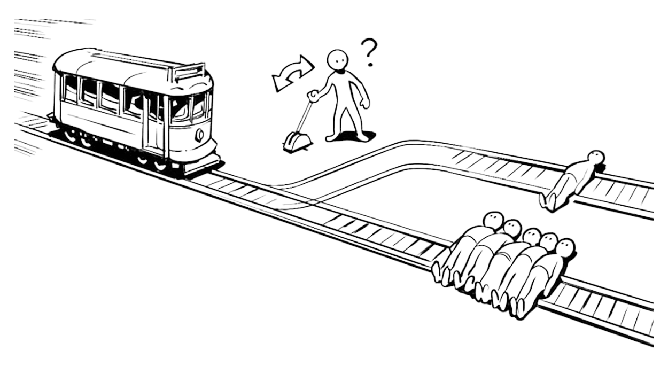
\includegraphics[width = 0.9\textwidth, height = 1.7cm]{img/trolley_problem.png}    
        \end{minipage}
        \begin{minipage}{0.6\textwidth}
            \textbf{The Trolley Problem:} Divert trolley to save many lives but sacrifice one? \\
            \textbf{Mathematics:} Develop models, quantify harm, compare consequences
        \end{minipage}
    \end{block}
    \vspace{0cm}

    \begin{block}{International Relations}
        \begin{minipage}{0.65\textwidth}
            % Game theory is applied to model interactions between countries in international relations. \\
            \textbf{The Game of Chicken:} Avoid disastrous outcomes while standing firm on demands. \\
            % Some examples: 
            % \begin{itemize}[leftmargin = 0.5cm, label = $\bullet$]
            %     \item The Cuban missile crises (1962)
            %     \item The Iran--USA hostage crisis (1979--1981)
            % \end{itemize}
            \textbf{Mathematics:} Predict outcomes, calculate risks, compute payoffs, and use game theory to navigate conflicts. 
        \end{minipage}
        \hspace{0.1cm}
        \begin{minipage}{0.3\textwidth}
            \centering
            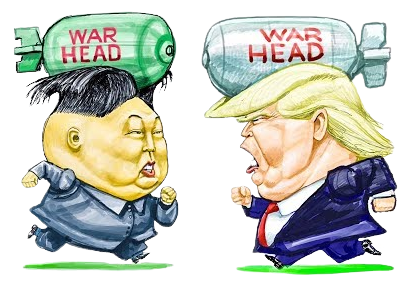
\includegraphics[width = 0.95\textwidth, height = 1.7cm]{img/chicken-game.png}    
        \end{minipage}
    \end{block}

    \begin{block}{Finance}
        \begin{minipage}{0.35\textwidth}
            \centering
            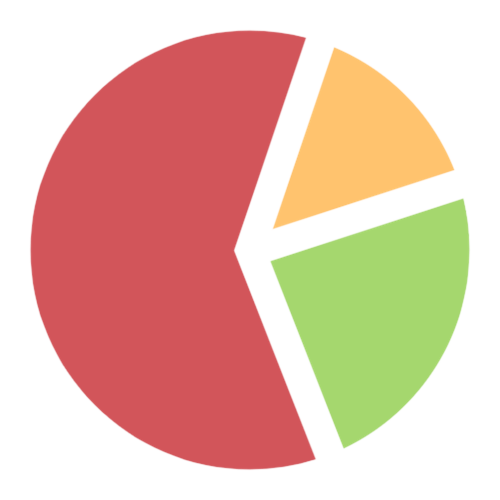
\includegraphics[width = 0.9\textwidth, height = 1.7cm]{img/piechart.png}
        \end{minipage}
        \begin{minipage}{0.6\textwidth}
            \textbf{Optimal portfolio:} Determine the best allocation of investments \\
            \textbf{Mathematics:} model dynamics, optimize profit.
        \end{minipage}
    \end{block}
    
\end{frame}


% \begin{frame}{Mathematics in Philosophy, Politics, and Economics}

    
%         \begin{minipage}{0.31\textwidth}
%         \begin{block}{Ethics}
%             {\centering
%             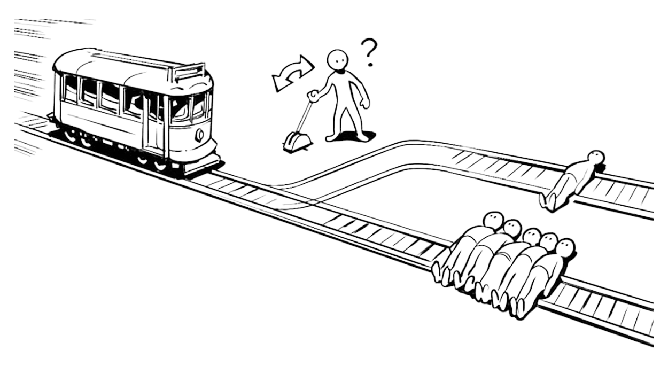
\includegraphics[width = 0.9\textwidth]{img/trolley_problem.png}}
%             \vspace{0.2cm}

%             \textbf{The Trolley Problem:} Divert trolley to save many lives but sacrifice one?
%             % \textbf{Mathematics:} Develop models, quantify harm, compare consequences
%             % Mathematical models can be used to analyze and make decisions in ethical dilemmas involving resource allocation, distribution of goods, or decision-making in complex moral contexts
%         \end{block}
%         \end{minipage}
%         \begin{minipage}{0.32\textwidth}
%         \begin{block}{International Relations}
%             {\centering
%             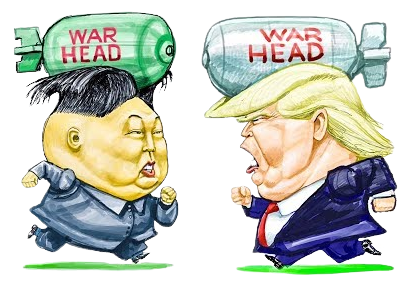
\includegraphics[width = 0.9\textwidth]{img/chicken-game.png}}
%             \vspace{0.2cm}
                      
%             \textbf{The Game of Chicken:} Avoid disastrous outcomes while standing firm on demands.
%             % \begin{itemize}[leftmargin = 0.5cm, label = $\bullet$]
%             %     \item The Cuban missile crises (1962)
%             %     \item The Iran--USA hostage crisis (1979--1981)
%             % \end{itemize}
%             % \textbf{Mathematics:} Predict outcomes, calculate risks, compute payoffs, and use game theory to navigate conflicts. 
%         \end{block}
%         \end{minipage}
%         \begin{minipage}{0.31\textwidth}
%         \begin{block}{Finance}
%             {\centering
%             \hspace{0.3cm} 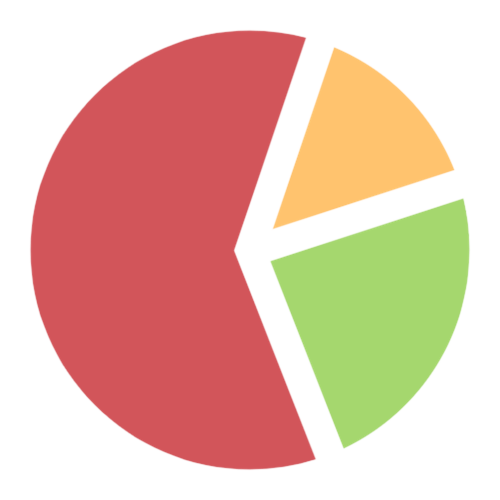
\includegraphics[height = 0.9\textwidth, height = 2.5cm]{img/piechart.png}}
%             \vspace{0.2cm}

%             \textbf{Optimal portfolio:}     
%             Determine the best allocation of investments. \\
%             % Mathematical models can be used to analyze and make decisions in ethical dilemmas involving resource allocation, distribution of goods, or decision-making in complex moral contexts
%         \end{block}
%         \end{minipage}
%         % \begin{minipage}{0.6\textwidth}
%          % \\
%         % \textbf{The Trolley Problem:} Divert trolley to save many lives but sacrifice
%         % one? What if that one is Steve Jobs?\\
%         % \textbf{Mathematics:} Develop models, quantify harm, compare consequences
%         % \end{minipage}

%     % \begin{block}{Logic}
%     %     \begin{minipage}{0.35\textwidth}
%     %         \centering
%     %         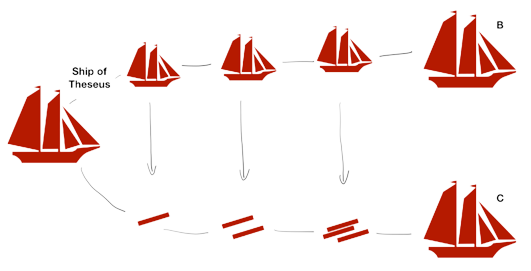
\includegraphics[width = 0.9\textwidth]{img/theseus-paradox.png}    
%     %     \end{minipage}
%     %     \begin{minipage}{0.6\textwidth}
%     %         By employing logical rules, philosophers can assess the logical structure and coherence of arguments, identifying any fallacies or inconsistencies \\
%     %         \textbf{The Ship of Theseus Paradox:}  If all the parts of a ship are replaced over time, is it still the same ship? \\
%     %         \textbf{Mathematics:} Logical arguments to analyze the relation between identity, change, and persistence.
%     %     \end{minipage}
%     % \end{block}
    
% \end{frame}

% \begin{frame}{Mathematics in Politics, Philosophy, and Economics}

%     \begin{block}{Voting Systems}
%         \begin{minipage}{0.35\textwidth}
%             \centering
%             {\LARGE Arrow's Theorem}
%             \vspace{-1cm} 
            
%             
\includegraphics[width = 0.9\textwidth]{img/voting2.png}    
%             \vspace{-1cm}
            
%             Given more than 2 choices, \\
%             no system can have \\ 
%             all the attributes of an \\
%             ideal voting system at once
%         \end{minipage}
%         \begin{minipage}{0.6\textwidth}
%             Mathematics is used to analyze various voting systems for fairness and efficiency, as well as their capacity to reflect voter preferences and minimize undesirable outcomes \\
%             \textbf{Arrow's Impossibility Theorem:} No system can satisfy all of these (desirable) attributes at once: 
%             \begin{itemize}[leftmargin = 0.3cm, label = $\bullet$]
%                 \item \textbf{Unrestricted Domain:} everyone's voice matters 
%                 \item \textbf{Non-Dictatorship:} no one can control everyone
%                 \item \textbf{Pareto Efficiency:} if everyone likes choice A over choice B, A should win
%                 \item \textbf{Independence of Irrelevant Alternatives:} adding new options should not change the result
%             \end{itemize}
%             \textbf{Mathematics:} Using set theory and logical reasoning one can demonstrate that these criteria contradict each other
%         \end{minipage}
%         \vspace{0.1cm}
        
%     \end{block}
    
% \end{frame}

% \begin{frame}{Mathematics in Politics}
    
%     \begin{block}{International Relations}
%         \begin{minipage}{0.35\textwidth}
%             \centering
%             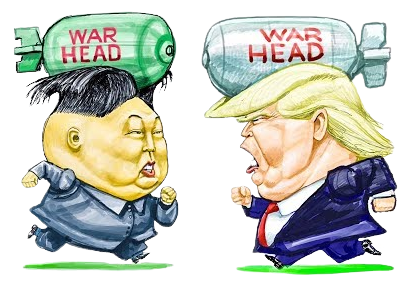
\includegraphics[width = 0.9\textwidth]{img/chicken-game.png}    
%         \end{minipage}
%         \begin{minipage}{0.6\textwidth}
%             Game theory is applied to model interactions between countries in international relations. \\
%             \textbf{The Game of Chicken:} Avoid disastrous outcomes while standing firm on demands. Some examples: 
%             \begin{itemize}[leftmargin = 0.5cm, label = $\bullet$]
%                 \item The Cuban missile crises (1962)
%                 \item The Iran--USA hostage crisis (1979--1981)
%             \end{itemize}
%             \textbf{Mathematics:} Predict outcomes, calculate risks, compute payoffs, and use game theory to navigate conflicts. 
%         \end{minipage}
%     \end{block}

%     \begin{block}{Other Applications}
%         \begin{itemize}[leftmargin = 0.5cm, label = $\bullet$]
%                 \item Campaign Strategy: optimize resource allocation for effective campaigns
%                 \item Social Network Analysis: study political influence and polarization
%                 \item Election Forecasting: predict election outcomes using statistics
%                 \item Budget Allocation: optimizes public fund distribution
%             \end{itemize}
%     \end{block}
    
% \end{frame}

% \begin{frame}{Mathematics in Economics}

%     ``It is clear that economics, if it is to be a science at all, must be a mathematical
%     science'' —William Stanley Jevons (1835--1882)
    
%     \begin{block}{Optimal Portfolio}
%         \vspace{-0.1cm}
        
%         \begin{minipage}{0.3\textwidth}
%             \centering
%             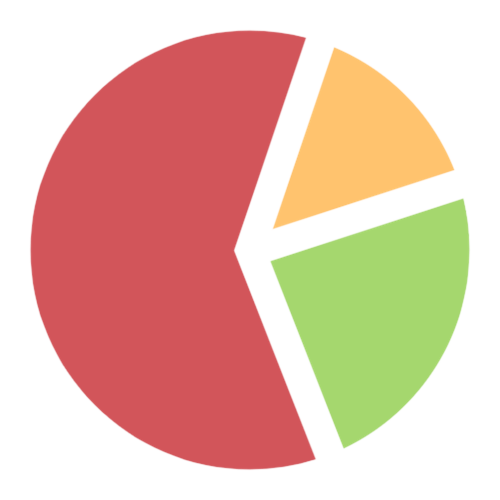
\includegraphics[width = 0.9\textwidth, height = 3.2cm]{img/piechart.png}    
%         \end{minipage}
%         \begin{minipage}{0.65\textwidth}
%             Determine the best allocation of investments among different assets to maximize returns and control the risk \\
%             \textbf{Mathematics:}
%             \begin{itemize}[leftmargin = 0.5cm, label = $\bullet$]
%                 \item Mathematical models capture the assets' dynamics
%                 \item Linear algebra is used to represent the problem
%                 \item Optimization techniques to find the optimal balance
%             \end{itemize}
%         \end{minipage}
%     \end{block}

%         \begin{block}{Other Applications}
%             \begin{itemize}[leftmargin = 0.5cm, label = $\bullet$, rightmargin = 0.2cm]
                
%                 \item \textbf{Supply and Demand Analysis:} Understand the price-supply-demand connection

%                 \item \textbf{Optimization Theory:} Maximize profits and minimize losses under constrains

%                 \item \textbf{Interest Rate Modeling:} Understand borrowing and lending

%                 \item \textbf{Econometric Analysis:} Test ideas and predict outcomes
%         \end{itemize}
%         \end{block}
    
% \end{frame}

\begin{frame}{Course topics}
    
    \begin{block}{Module 1: Elements of Mathematics}
        \begin{minipage}{0.35\textwidth}
            \centering
            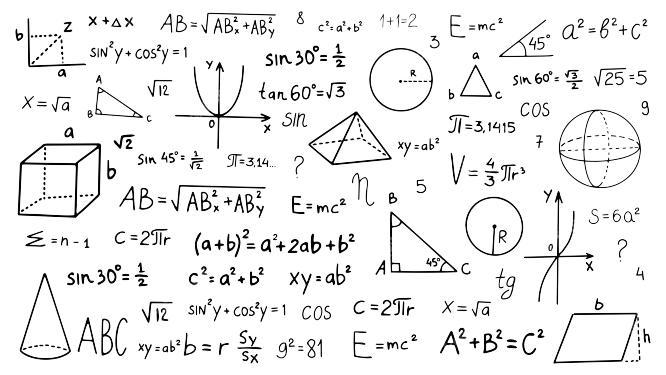
\includegraphics[width = 0.9\textwidth]{img/basic-math.png}    
        \end{minipage}
        \begin{minipage}{0.6\textwidth}
            \begin{itemize}[leftmargin = 0.5cm, label = $\bullet$]
            \item Introduction to basic concepts of general mathematics: \Corange{numbers}, \Corange{sets}, \Corange{sequences}, \Corange{functions}, \Corange{graphs}, \Corange{limits}, and others. 
            \end{itemize}
            %This part of the course lays down the foundations required to explore more sophisticated ideas.
        \end{minipage}
    \end{block}

    \begin{block}{Module 2: Differential calculus}
        \begin{minipage}{0.35\textwidth}
            \centering
            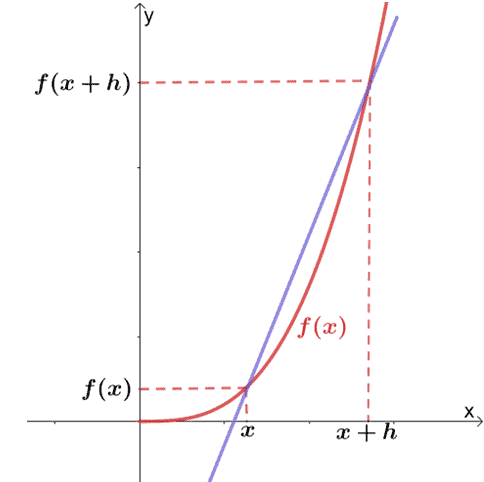
\includegraphics[width = 0.9\textwidth,height=3cm]{img/derivative.png}    
        \end{minipage}
        \begin{minipage}{0.6\textwidth}
            \begin{itemize}[leftmargin = 0.5cm, label = $\bullet$]
            \item Definition of the \Corange{derivative} of a function and rules to compute it. 
            \item Applications of derivatives to compute \Corange{slopes} of functions, solve \Corange{optimization} problems, and understand economic concepts.
            \end{itemize}
        \end{minipage}
    \end{block}

\end{frame}

\begin{frame}{Course topics}
    
    \begin{block}{Module 3: Integral calculus}
        \begin{minipage}{0.35\textwidth}
            \centering
            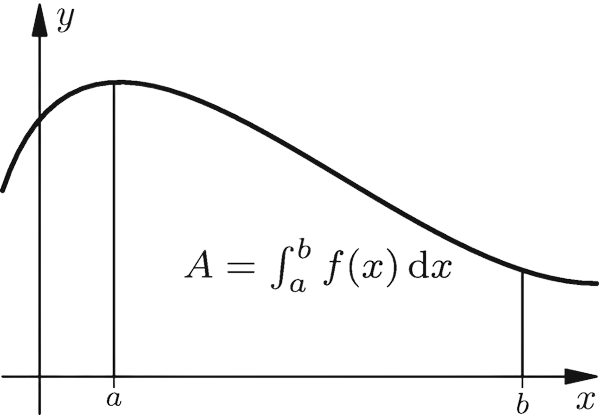
\includegraphics[width = 0.9\textwidth]{img/integral.png}    
        \end{minipage}
        \begin{minipage}{0.6\textwidth}
            \begin{itemize}[leftmargin = 0.5cm, label = $\bullet$]
            \item Definition of the \Corange{integral of a function} and techniques to compute it. 
            \item Applications of integrals to compute \Corange{areas} bounded by curves and to solve economic problems.
            \end{itemize}
        \end{minipage}
    \end{block}

    \begin{block}{Module 4: Methods of linear algebra}
        \begin{minipage}{0.35\textwidth}
            \centering
            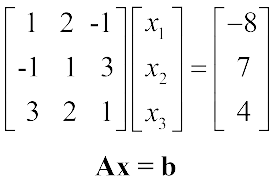
\includegraphics[width = 0.9\textwidth]{img/linear.png}    
        \end{minipage}
        \begin{minipage}{0.6\textwidth}
            \begin{itemize}[leftmargin = 0.5cm, label = $\bullet$]
            \item The study of systems of \Corange{linear equations} and the use of matrices to this end: \Corange{matrix notation}, % of a system of linear equations, 
            \Corange{matrix algebra}, and others.
            %classification of a system of linear equations in terms of their solutions.
            \end{itemize}
        \end{minipage}
    \end{block}
    
\end{frame}

\begin{frame}{Course topics (if time allows)}
    
    \begin{block}{Module 5: Recurrence equations and Ordinary differential equations}
        \begin{minipage}{0.35\textwidth}
            \centering
            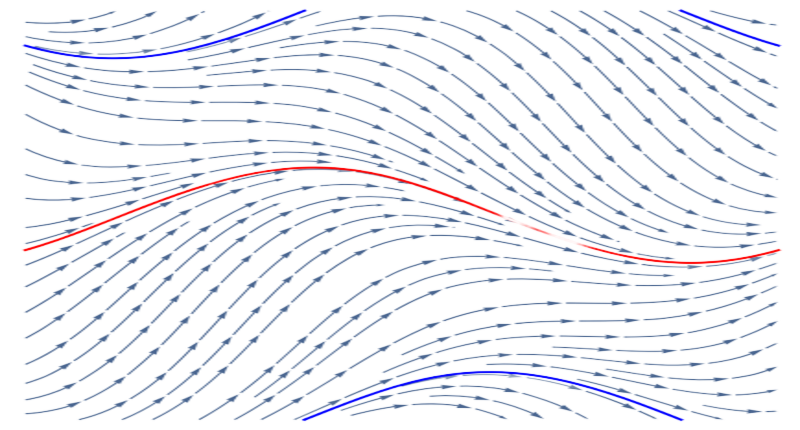
\includegraphics[width = 0.9\textwidth]{img/ODE2.png}    
        \end{minipage}
        \begin{minipage}{0.6\textwidth}
            \begin{itemize}[leftmargin = 0.5cm, label = $\bullet$]
            \item The study of equations that relates a term of a sequence to the previous terms. 
            %Homogeneity and initial conditions. Application to economics.
            \item The study of equations that relate a function to its derivatives. 
            %Order, Homogeneity, and initial conditions. Techniques and analysis of solutions. Applications to economics.
            \end{itemize}
        \end{minipage}
    \end{block}
    
\end{frame}

% \begin{frame}{Time table}

%     {\hspace{0.04cm}
%     \begin{minipage}{0.7\textwidth}
%         \begin{block}{\centering Time plan (It may change)}
%             \vspace{0.15cm}
            
%             \begin{itemize}[leftmargin = 0.2cm, label = ]
%                 \item \textbf{Week 1-2:} Elementary Mathematics
%                 \item Quiz
%                 \item \textbf{Week 3-4:} Differential Calculus
%                 \item \textbf{Week 5-6:} Differential Calculus / Integral Calculus
%                 \item \textbf{Week 7-8:} Integral Calculus 
%                 \item First midterm (Calculus)
%                 \item \textbf{Week 9-10:} Linear Algebra
%                 \item \textbf{Week 11-12:} Recurrence Equations
%                 \item Second midterm (Linear Algebra + Recurrence Equations)
%                 \item \textbf{Week 13-14:} Ordinary Differential Equations
%                 \item Final exam :)
%             \end{itemize}
%         \end{block}
    
%     \end{minipage}\hspace{0.25cm}
%     \begin{minipage}{0.25\textwidth}
%         \vspace{-0cm}
        
%         \begin{block}{\centering Typical week}
%             \vspace{0.15cm}
            
%             \begin{itemize}[leftmargin = 0.2cm, label = , rightmargin = 0.2cm]
%                 \item \textbf{Monday} - 10:00 \\
%                 Theory
%                 \item \textbf{Wednesday} - 11:00 \\
%                 Theory / Practice
%                 \item \textbf{Friday} - 10:00 \\
%                 Practice
%             \end{itemize}
%         \end{block}
%         \vspace{0.3cm}

%         {\hspace{0.14cm} 
\includegraphics[width = 0.9\textwidth]{img/time-plan.png}}
%     \end{minipage}
%     }
    
% \end{frame}

\begin{frame}{Recommended resources}

    \begin{block}{\href{https://www.maplesoft.com/products/Maple/students/}{Maple}}
        \begin{minipage}{0.35\textwidth}
            \centering
            
\includegraphics[width = 0.9\textwidth]{img/logo-Maple.png}    
        \end{minipage}
        \begin{minipage}{0.6\textwidth}
            Software that performs
            %that empowers users to \Corange{explore and solve} complex mathematical problems. It offers a \Corange{user-friendly} environment for performing 
            \Corange{symbolic and numerical calculations}, and creates interactive visualizations. \\
            \textbf{Availability:} Free for CUNEF students   
        \end{minipage}
    \end{block}

    \begin{block}{\href{https://www.desmos.com/}{Desmos}}
        \begin{minipage}{0.35\textwidth}
            \centering
            
\includegraphics[width = 0.9\textwidth]{img/146-1466450_desmos-geometry-desmos-symbol-removebg-preview.png}    
        \end{minipage}
        \begin{minipage}{0.6\textwidth}
            Online graphing calculator that helps \Corange{visualize graphs and functions}. 
            %It can plot graphs, create tables, and even animate functions. 
            \\
            \textbf{Availability:} Free
        \end{minipage}
    \end{block}

    \begin{block}{\href{https://www.desmos.com/}{ChatGPT}}
        \begin{minipage}{0.35\textwidth}
            \centering
            
\includegraphics[width = 0.9\textwidth]{img/chatGPT.png}  
        \end{minipage}
        \begin{minipage}{0.6\textwidth}
            \Corange{Generative artificial intelligence} chatbot (other generative AIs like Gemini and Grok also work).  
            %It can plot graphs, create tables, and even animate functions. 
            \\
            \textbf{Availability:} Free (+ paid Pro version) \\
        \end{minipage}
    \end{block}
    
    % \begin{block}{\href{https://www.wolframalpha.com/}{Wolfram Alpha}}
    %     \begin{minipage}{0.35\textwidth}
    %         \centering
    %         
\includegraphics[width = 0.9\textwidth]{img/623b006d27d4946aceae2fd9.png}    
    %     \end{minipage}
    %     \begin{minipage}{0.6\textwidth}
    %         \Corange{Computational knowledge engine} that helps with a wide range of mathematical problems. It can perform \Corange{symbolic and numerical computations}, algebraic manipulations, solve equations, and even provide \Corange{step-by-step solutions} to problems. \\
    %         \textbf{Availability:} Free (+ paid Pro version)
    %     \end{minipage}
    % \end{block}

\end{frame}

% \begin{frame}{Recommended resources}

%     \begin{block}{\href{https://www.desmos.com/}{Desmos}}
%         \begin{minipage}{0.35\textwidth}
%             \centering
%             
\includegraphics[width = 0.9\textwidth]{img/146-1466450_desmos-geometry-desmos-symbol-removebg-preview.png}    
%         \end{minipage}
%         \begin{minipage}{0.6\textwidth}
%             \Corange{Online graphing calculator} that helps us \Corange{visualize mathematical concepts and functions}. It can plot graphs, create tables, and even animate functions. \\
%             \textbf{Availability:} Free
%         \end{minipage}
%     \end{block}

%     % \begin{block}{\href{https://math.stackexchange.com/}{Math StackEchange}}
%     %     \begin{minipage}{0.35\textwidth}
%     %         \centering
%     %         
\includegraphics[width = 0.9\textwidth]{img/LogoEmail.png}    
%     %     \end{minipage}
%     %     \begin{minipage}{0.6\textwidth}
%     %         An \Corange{online platform} that serves as a \Corange{hub for people interested in mathematics}. It offers a space where users can \Corange{seek help}, \Corange{share knowledge}, and engage in discussions related to a wide range of mathematical concepts and problems. \\
%     %         \textbf{Availability:} Free
%     %     \end{minipage}
%     % \end{block}
    
% \end{frame}

% \begin{frame}{Recommended resources}
    
%     \begin{block}{\href{https://brilliant.org/courses/\#/math}{Brilliant.org}}
%         \begin{minipage}{0.35\textwidth}
%             \centering
%             
\includegraphics[width = 0.9\textwidth]{img/l_create_Logo_Black_Vertical_Large.png}    
%         \end{minipage}
%         \begin{minipage}{0.6\textwidth}
%             An \Corange{online education platform} known for its engaging and \Corange{effective mathematics courses}. These courses are crafted to foster a \Corange{deep understanding} of foundational topics as well as advanced areas of mathematics, and to develop robust \Corange{problem-solving skills}. \\
%             \textbf{Availability:} Free (+ paid Pro version)
%         \end{minipage}
%     \end{block}
    
% \end{frame}

\begin{frame}
\frametitle{Recommended Bibliography}
\begin{minipage}{0.65\textwidth}
        
    \begin{enumerate}[label=$\bullet$,leftmargin=0.4cm,rightmargin=0.4cm]
        \item You can find a comprehensive bibliography list in the syllabus

        \item The recommended bibliography emphasizes the applicability to economic contexts.

        \item We will mostly follow the book \\
        \faBook\quad \Corange{\textbf{Mathematics for economics and finance: methods and modeling}}, by Anthony and Biggs.
    \end{enumerate}
    \end{minipage}
    \hspace{0.4cm}
    \begin{minipage}{0.3\textwidth}
        \centering
        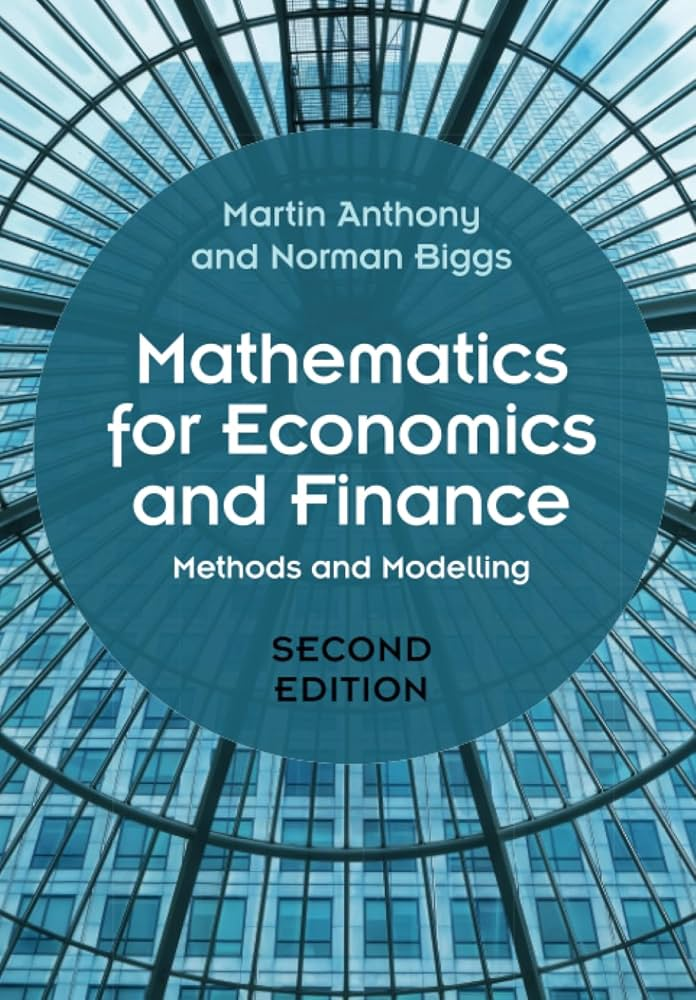
\includegraphics[width=\linewidth]{img/mathematics_for_economics.jpg}
        \href{https://encuentra.cunef.edu/permalink/34CUNEF_INST/3hqjvi/alma991000200539708131}{Grab your copy!}
    \end{minipage}
\end{frame}


% \begin{frame}{Recommended bibliography}

    
%     \begin{itemize}[leftmargin = *, label= $ $]
%         \item \faBook\quad \Corange{\textbf{Mathematics for economics and finance: methods and modelling}}  \\ Anthony, M. and Biggs, N.
        
%         \item \faBook\quad \textbf{Essential mathematics for economic analysis} \\
%         Sydsæter, K., Hammond, P., Strøm, A., and Carvajal A.
        
%         \item \faBook\quad \textbf{Mathematics for economics and business} \\
%         Jacques, I.         
        
%         \item \faBook\quad \textbf{Maths for Economics} \\
%         Renshaw, G. \\
        
%         \item \faBook\quad \textbf{An introduction to mathematics for economics} \\ 
%         Asano, A.        
        
%         \item \faBook\quad \textbf{Fundamental Methods of Mathematical Economics} \\
%         Chiang, A. C. and Wainwright, K.
        
%     \end{itemize}

% \end{frame}

% \begin{frame}{Achieving success}

%     Unlock your math potential with these core strategies.
    
%     \begin{itemize}[leftmargin = 0.5cm, label = $\bullet$]
%             \item \textbf{Practice regularly:} Consistent effort brings success
%             \item \textbf{Grasp concepts:} Understand why, not just how
%             % \item \textbf{Active learning:} Engage, explain, solve actively
%             \item \textbf{Early start:} Begin assignments and study ahead of time
%             \item \textbf{Use resources:} Use online tools, books, videos
%             \item \textbf{Foster curiosity:} Formulate questions and ask
%             \item \textbf{Seek help:} Use the office hours if needed \\ (online meeting upon agreement via email)
%             \item \textbf{Enjoy!} 
%     \end{itemize}
    
% \end{frame}

% \begin{frame}{Assessment and grading}

%     % \begin{itemize}[leftmargin=*,label=$\bullet$]
%     %     \item AR: attendance rate
%     %     \item M1: 1st midterm
%     %     \item M2: 2nd midterm
%     %     \item Q: quiz
%     %     \item GW: group work
%     %     \item CE: continuous evaluation
%     %     \item FE: final exam
%     %     \item RE: result exam
%     %     \item FG: final grade
%     % \end{itemize}

% \begin{center}
% \vspace{-0.15cm}

% \begin{frame}{About me}

%     \begin{block}{Education}
%          \begin{minipage}{0.5\textwidth}
%             \begin{itemize}[leftmargin = 0.5cm, label = $\bullet$]
%                 \item \textbf{Bachelor degree:} \\
%                 Mathematics \\
%                 Universidad de La Habana
%                 \item \textbf{MSc and PhD:} \\
%                 Mathematical Engineering \\
%                 Universidad Carlos III de Madrid
%             \end{itemize}     
%          \end{minipage}
%          \begin{minipage}{0.45\textwidth}
%              
\includegraphics[height = 2.5cm]{img/acronimo_nombrevertical.png}
%              \quad\quad 
%              
\includegraphics[height = 2.5cm]{img/logo-UH.pdf}
%          \end{minipage}
         
%     \end{block}

%     \begin{block}{Research}
%          \begin{itemize}[leftmargin = 0.5cm, label = $\bullet$]
%             \item Optimal Stopping Problems 
%             \item Renewal Energy
%         \end{itemize} 
%     \end{block}

% \end{frame}

% \begin{frame}{About you}

%     \begin{block}{Introduce yourself}
%         Introduce yourself in a short video and upload it to this task already created in Canvas. You can talk about:

%         \begin{itemize}[leftmargin = 0.5cm, label = $\bullet$, rightmargin = 0.2cm]
%             \item Name? Where are you from?
%             \item Educational background, with an emphasis on mathematics
%             \item Expectations/preferences about this course
%             \item Why you decided to study PPE?
%             \item Preferred ways to asses your knowledge (quizzes, projects, exams, talks, peer review tasks, individual vs group works, student-generated questions...)
%             \item Interests outside mathematics
%         \end{itemize}
%     \end{block}
    
% \end{frame}

\begin{frame}{Assessing your math level}

    % \begin{block}{Assessment quizzes}
        \begin{itemize}[label=$\bullet$]
            \item \textbf{You will take three quizzes} in Canvas to assess your math level
            \begin{enumerate}[label=$+$]
                \item Arithmetic Quiz
                \item Basic Algebra and Quantitative Reasoning Quiz
                \item Algebra and Functions Quiz
            \end{enumerate}
    
            \item The assessment quizzes are \textbf{not gradable}.
            
            \item The goal is to \textbf{spot your weaknesses} and strengthen those areas

            \item You will not need to have Proctorio installed for these quizzes
        \end{itemize}
    % \end{block}
    
\end{frame}

% \begin{frame}{Open Q\&A}

%     \centering Time to ask!
    
% \end{frame}


\end{document}